\subsection{The computer time}

\subsection{The error}

Too find out how the error developed with the number of mesh points, the step length, we calculated the maximum relative error with different step lengths. The results from these calculations are in Tb. \ref{tab:error_developement} and in Fig. \ref{fig:error_development}. 

\begin{table}[H]\caption{This is a table listing the log of the error and the log of the associated $h$ value. We can see that the smallest error, log(RelativeError) $= -7$, is accomplished when $\log(h) = -4$.}\label{tab:error_developement}
\begin{tabular}{cc}
log(h): & log(RelativeError): \\ \hline
-1.04 & -1.18 \\  \hline
-2.00 & -3.09 \\  \hline
-3.00 & -5.08 \\  \hline
-4.00 & -7.09 \\  \hline
-5.00 & -6.57 \\  \hline
-6.00 & -4.65 \\  \hline
-7.00 & -2.73 \\  \hline

\end{tabular}
\end{table}

\begin{figure}[H]
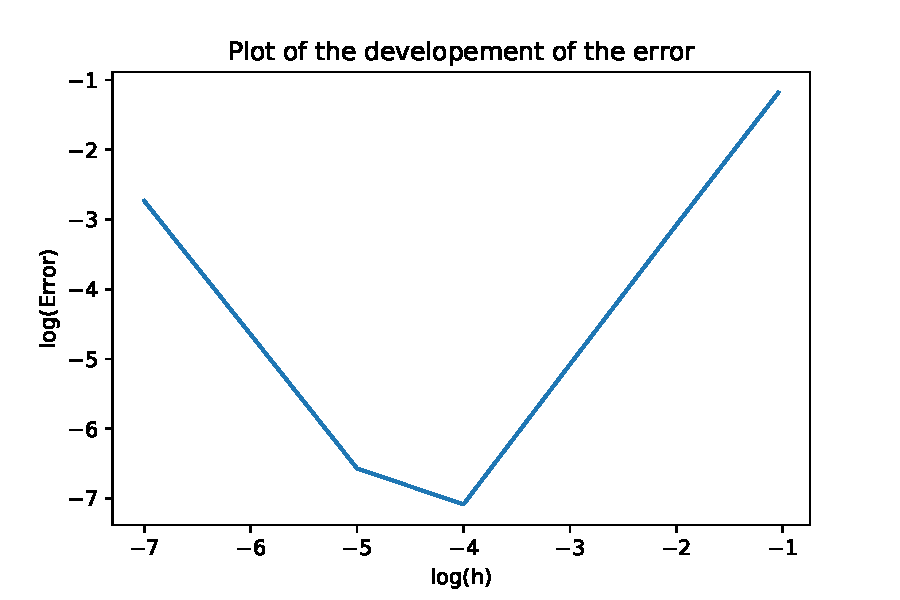
\includegraphics[width=\linewidth]{figures/ErrorDevelopement.pdf}\caption{This is a plot of the log of the error versus the log of the associated $h$ value. We can see that the smallest error, log(RelativeError) $= -7$, is accomplished when $\log(h) = -4$.}\label{fig:error_development}
\end{figure}
